\documentclass[]{standalone}

\begin{document}
	\begin{frame}{Results}{\textbf{Pre}-Processing}
	\vspace{-28pt}
	
	\begin{columns}
		\begin{column}{0.35\textwidth}
		\begin{itemize}
	
		\item Comparison with masks obtained with FSL;
		\item Computed metric: Dice Similarity Coefficient;
	\end{itemize}
		\end{column}
		
		\begin{column}{0.65\textwidth}
		\begin{block}{Dice Similarity Coefficient}
		\begin{table}[h!]
			\centering
			\small
			\setlength{\tabcolsep}{3pt}
			\begin{tabular}{c|cccc}
					    & \textbf{Mean} & \textbf{Std. Dev.} & \textbf{Median} & \textbf{IQR} \\ \hline
			\textbf{Brain Mask} & 0.87          & 0.12               & 0.93            & 0.11         \\
			\textbf{WM}         & 0.78          & 0.19               & 0.83            & 0.19         \\
			\textbf{GM}         & 0.67          & 0.30               & 0.80            & 0.28         \\
			\textbf{CSF}        & 0.66          & 0.24               & 0.79            & 0.22        
			\end{tabular}
			\end{table}
			\vspace{-10pt}
		\end{block}
			\vspace{-5pt}
			\begin{figure}[h!]
			\tiny
			\centering
				\begin{subfigure}{0.3\textwidth}
					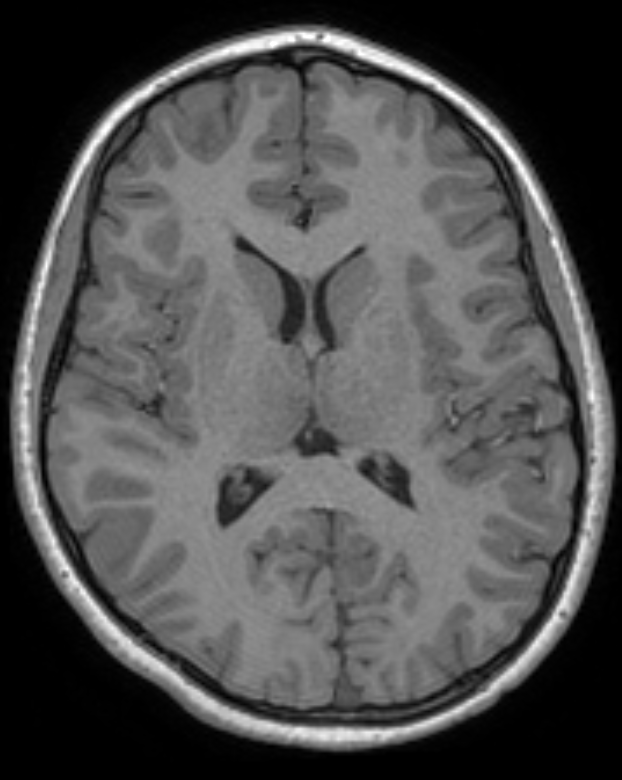
\includegraphics[scale=0.11]{./IMG/T1W48.png}
					\caption*{\tiny T1W }
				\end{subfigure}
				\hfill
				\begin{subfigure}{0.3\textwidth}
					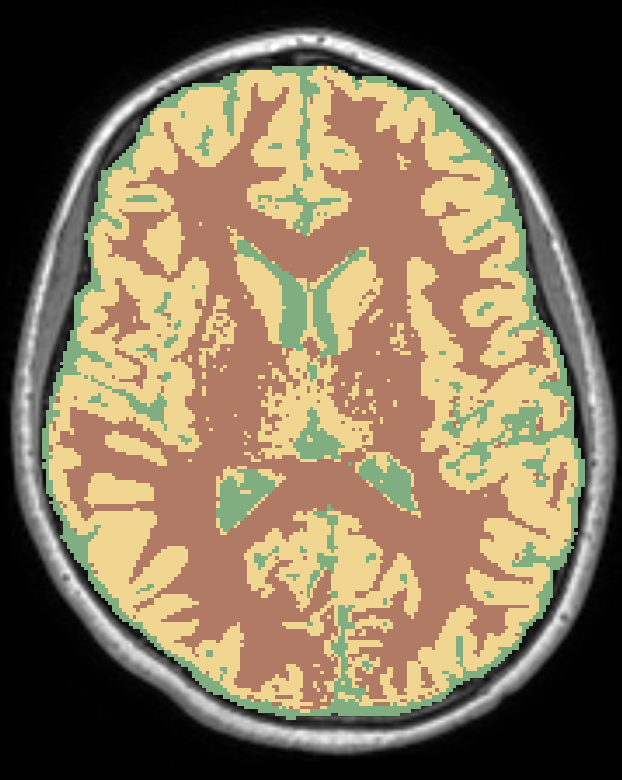
\includegraphics[scale=0.11]{./IMG/FSL_SEG48.png}
					\caption*{\tiny FSL}
				\end{subfigure}
				\hfill
				\begin{subfigure}{0.3\textwidth}
					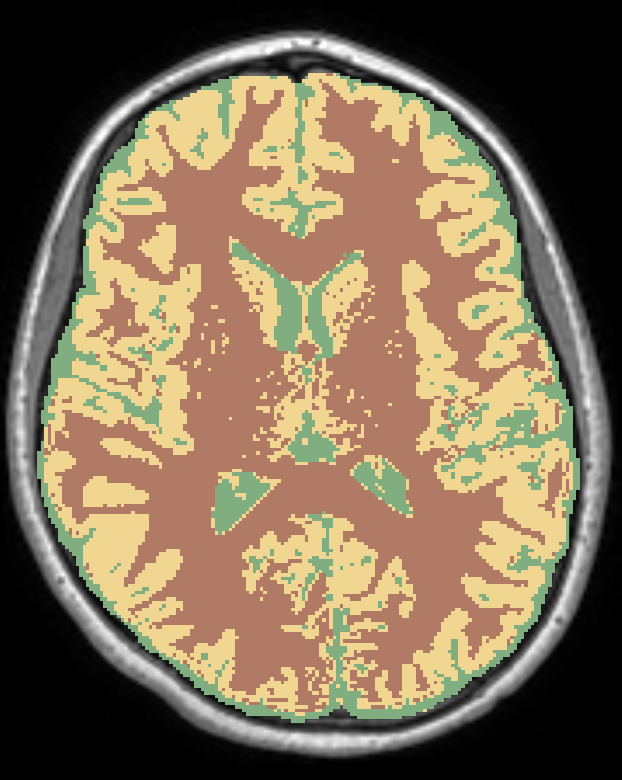
\includegraphics[scale=0.11]{./IMG/SEG48.png}
					\caption*{\tiny Pipeline}
				\end{subfigure}
			\end{figure}
		\end{column}
	\end{columns}
	
	\end{frame}
\end{document}
